% !TEX root = task-1-16-2.tex
% Editable task bank. Append new BankTask blocks at the end of the document.
\documentclass[12pt,a4paper]{article}
\usepackage{physics-textbook}
\usepackage{graphicx,needspace}
\usetikzlibrary{decorations.pathmorphing}
\newif\ifShowSolutions
\ifdefined\TutorEdition
  \ShowSolutionstrue
\else
  \ShowSolutionsfalse % Change to \ShowSolutionstrue to display solutions.
\fi
\newcounter{banktask}
\newsavebox{\BankTaskBox}
\newcommand{\BankTaskContent}[3]{%
  \noindent\textbf{\thebanktask.}\quad #2\par
  \ifShowSolutions
    \Needspace{50mm}% Keep the solution heading with its opening text or diagram.
    #3\par
    \ifdefined\TutorEdition
      \ifcsname TutorSource#1\endcsname
        \nopagebreak\smallskip{\small\csname TutorSource#1\endcsname\par}%
      \fi
    \fi
  \fi
}
\newcommand{\BankTask}[3]{%
  \refstepcounter{banktask}\par\medskip
  \sbox{\BankTaskBox}{\begin{minipage}{\linewidth}%
    \BankTaskContent{#1}{#2}{#3}\end{minipage}}%
  \ifdim\dimexpr\ht\BankTaskBox+\dp\BankTaskBox\relax>\dimexpr\textheight-20mm\relax
    \Needspace{35mm}\BankTaskContent{#1}{#2}{#3}%
  \else
    \Needspace{\dimexpr\ht\BankTaskBox+\dp\BankTaskBox\relax}%
    \noindent\usebox{\BankTaskBox}\par
  \fi
  \medskip
}
\begin{document}
\BookSubsection{1.16.2}{Неподвижный блок}


% Source 41563: https://phys-ege.sdamgia.ru/problem?id=41563
\BankTask{41563}{
\begin{center}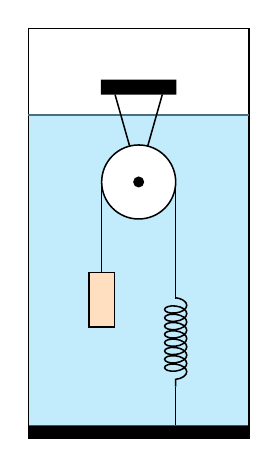
\begin{tikzpicture}[>=stealth,line width=.55pt]\fill[cyan!24](0,0)rectangle(2.8,4.1);\draw(0,0)rectangle(2.8,5.2);\draw[cyan!45!black](0,4.1)--(2.8,4.1);\fill(0,0)rectangle(2.8,.16) (.92,4.36)rectangle(1.88,4.55);\draw(1.1,4.36)--(1.4,3.3)--(1.7,4.36);\draw[fill=white](1.4,3.25)circle(.47);\fill(1.4,3.25)circle(.07);\draw(.93,3.25)--(.93,2.1) (1.87,3.25)--(1.87,1.77);\draw[fill=orange!25](.77,1.41)rectangle(1.09,2.1);\draw[decorate,decoration={coil,segment length=3pt,amplitude=4pt}](1.87,1.78)--(1.87,.65);\draw(1.87,.65)--(1.87,.16);\end{tikzpicture}\end{center}На рисунке представлена система тел, состоящая из неподвижного блока с перекинутой через него лёгкой и нерастяжимой нитью, к концам которой привязаны груз массой m  =  $0{,}8\,\text{кг}$ и объёмом V  =  $100\,\text{см}^{3}$ и лёгкая пружина жёсткостью k  =  $100$ H/м. Эта система находится в покое и  погружена в сосуд с жидкостью плотностью $\rho = 900\,\text{кг/м} ^3 .$ Нижний конец пружины прикреплён к дну сосуда. Как и на сколько изменится сила натяжения нити, действующая на пружину, если сосуд будет заполнен не первоначальной жидкостью, а таким же объёмом воды? Считать, что трение в оси блока отсутствует.
}{
\smallskip\noindent\textbf{Решение}\par
\begin{center}\begin{tikzpicture}[>=stealth,line width=.55pt]\fill[cyan!24](0,0)rectangle(2.8,4.1);\draw(0,0)rectangle(2.8,5.2);\draw[cyan!45!black](0,4.1)--(2.8,4.1);\fill(0,0)rectangle(2.8,.16) (.92,4.36)rectangle(1.88,4.55);\draw(1.1,4.36)--(1.4,3.3)--(1.7,4.36);\draw[fill=white](1.4,3.25)circle(.47);\fill(1.4,3.25)circle(.07);\draw(.93,3.25)--(.93,2.1) (1.87,3.25)--(1.87,1.77);\draw[fill=orange!25](.77,1.41)rectangle(1.09,2.1);\draw[decorate,decoration={coil,segment length=3pt,amplitude=4pt}](1.87,1.78)--(1.87,.65);\draw(1.87,.65)--(1.87,.16);\draw[->](-.25,5.18)--(-.25,.05)node[below]{$y$};\node[left]at(-.25,5.18){$0$};\draw[->](.93,1.77)--(.93,2.93)node[left]{$\vec T_1$};\draw[->](.93,1.77)--(.93,2.55)node[right]{$\vec F_{\text{арх}}$};\draw[->](.93,1.77)--(.93,.83)node[below]{$m\vec g$};\end{tikzpicture}\end{center}Изобразим силы, действующие на груз: сила тяжести $m\vec g,$ сила натяжения нити $\vec T_1,$ сила Архимеда $\vec F_A.$ По третьему закону Ньютона сила натяжения нити равна силе упругости, возникающей в пружине, равна силе натяжения $\vec T_1,$ так как нить легкая и сила трения в блоке отсутствует. В инерциальной системе отсчета, связанной с Землей, условие равновесия груза имеет вид:

\[m\vec g + \vec T_1 + \vec F_A=0.\]

В проекции на ось Oy: $T_1 + F_A - mg=0,$ где сила Архимеда равна $F_A=\rho gV.$ Откуда сила натяжения нити, действующая на груз, погруженный в жидкость, равна

\[T_1=mg - \rho gV.\]

Если  жидкость заменить на воду, то сила натяжения нити станет равной

\[T_2=mg - \rho_{\,\text{в}} gV.\]

Поскольку плотность воды  больше плотности жидкости, то сила Архимеда увеличится, а сила натяжения уменьшится на величину, равную

\[T_1 - T_2=gV ( \rho_{\,\text{в}} - \rho ) =10 \cdot 10 ^{ - 4 } \cdot ( 1000 - 900 ) =0{,}1\,\text{Н}.\]

Ответ: уменьшится на $0{,}1$ Н.
}

% Source 50800: https://phys-ege.sdamgia.ru/problem?id=50800
\BankTask{50800}{
\begin{center}\begin{tikzpicture}[task graph,>=stealth]\draw(-1.15,3.57)--(1.1,3.57);\foreach \x in {-1.1,-.8,...,1.0}{\draw(\x,3.57)--++(.24,.24);}\draw(0,3.57)--(0,2.18) circle(.75);\draw(-.75,2.18)--(-.75,-.20) (.75,2.18)--(.75,-.83);\draw[fill=gray!15](-1.29,-.96)rectangle(-.21,-.20)node[midway]{\(M\)};\draw[fill=gray!15](.22,-1.59)rectangle(1.28,-.83)node[midway]{\(M\)};\draw[fill=gray!30](.50,-.83)rectangle(1.0,-.38)node[midway,right,xshift=9pt]{\(m\)};\end{tikzpicture}\end{center}Два одинаковых бруска массой M  =  $500\,\text{г}$ связаны между собой невесомой нерастяжимой нитью, перекинутой через невесомый гладкий блок, неподвижно закреплённый на потолке (см. рис.). На один из блоков кладут груз массой m  =  $100\,\text{г}$, и система приходит в движение. С какой силой F груз будет давить на брусок? Сделайте схематический рисунок с указанием сил, действующих на бруски и груз. Обоснуйте применимость законов, используемых для решения задачи.
}{
\smallskip\noindent\textbf{Решение}\par
Обоснование. Cистему отсчета, связанную с Землей, будем считать инерциальной. Так как движение грузов поступательное, то их можно описывать моделью материальной точки. Значит, можно применять законы Ньютона для описания движения грузов. Нить, которая связывает тело массой М и тело массой M + m с перегрузком, является невесомой, а блок  — идеальным (его масса равна нулю, трением в его оси вращения можно пренебречь). Следовательно, на оба тела действует одинаковая по модулю сила натяжения нити. Кроме того, нить нерастяжима. Поэтому оба тела движутся с одинаковым по модулю ускорением.

\begin{center}\begin{tikzpicture}[task graph,>=stealth]\draw(-1.15,3.57)--(1.1,3.57);\foreach \x in {-1.1,-.8,...,1.0}{\draw(\x,3.57)--++(.24,.24);}\draw(0,3.57)--(0,2.18) circle(.75);\draw(-.75,2.18)--(-.75,-.20) (.75,2.18)--(.75,-.83);\draw[fill=gray!15](-.94,-1.07)rectangle(-.56,-.40)(.56,-1.66)rectangle(.94,-.7);\draw[->] (0,2.18)--(0,3.4) node[right]{\(\vec F\)};\draw[->] (0,2.18)--(0,.92) node[right]{\(\vec F\)};\draw[->] (-.75,2.18)--(-.75,.92) node[right]{\(\)};\draw[->] (.75,2.18)--(.75,.92) node[right]{\(\)};\draw[->] (-.75,-.73)--(-.75,.6) node[left]{\(\vec T_1\)};\draw[->] (.75,-1.2)--(.75,.35) node[right]{\(\vec T_2\)};\draw[->] (-.75,-.73)--(-.75,-1.69) node[left]{\(M\vec g\)};\draw[->] (.75,-1.2)--(.75,-2.4) node[right]{\((M+m)\vec g\)};\draw[->] (2.66,3.3)--(2.66,-1.42) node[right]{\(X\)};\end{tikzpicture}\end{center}
Перейдем к решению. Запишем, на основании второго закона Ньютона, уравнения движения для обоих грузов в проекции на вертикальную ось, направленную вниз (см. рис.):

$Ma_1=Mg - T_1,$ $( M + m ) a_2= ( M + m ) g - T_2.$

Здесь через $a_1$ и $a_2$ обозначены проекции ускорений грузов M и $( M + m )$ на вертикальную ось, а через $T_1$ и $T_2$  — проекции сил натяжения нити на ту же ось.
В силу условия задачи из-за нерастяжимости нити $a_1= - a_2= - a,$ а из-за невесомости блока и нити и отсутствия трения$T_1=T_2=T.$ 
Из написанных уравнений получаем: 

\[a= \frac{m}{m + 2M} g.\]

Рассмотрим движение только перегрузка. Он давит на груз силой, которая по третьему закону Ньютона равна $F=N.$ Запишем второй закон Ньютона для перегрузка в проекции на вертикальную ось:

\[mg - N=ma.\]

Тогда сила, с которой перегруз давит на груз при их движении, равна:

\[F=m ( g - a ) = \frac{2mMg}{m + 2M} = \frac{2 \cdot 10 \cdot 0{,}1 \cdot 0{,}5}{0{,}1 + 2 \cdot 0{,}5} \approx 0{,}91\,\text{Н}.\]

Ответ: $\approx 0{,}91\,\text{Н}.$
}

\end{document}
